
\chapter{Teoremi di Convergenza}

\section{Teoria}

\subsection{Campione Aleatorio Casuale}

Il modello probabilistico fondamentale per la statistica è la successione $\suc$ di variabili aleatorie \textbf{indipendenti ed identicamente distribuite} (v.a i.i.d.) \n

\ind \textbf{Definizione}: Chiameremo \textbf{campione aleatorio casuale} di ampiezza n le $\suc$ osservabili. \n 

\ind \textbf{Osservazione}: Uno dei pochi casi in cui è facile conoscere la distribuzione del campione aleatorio è il caso del \textbf{campione gaussiano} $\suc \sim N(\mu, \sigma^2)$ in quanto possiamo calcolare la media campionaria $\mc $ con la tavola della distribuzione. \n

\ind \textbf{Obiettivo}: Per ottenere il nostro obiettivo, ovvero quello di conoscere la distribuzione di un campione aleatorio $\suc$, dovremo ricondurre il campione aleatorio ad una gaussiano $N(0,1)$ \n

\ind \textbf{Definizione}: Per standardizzare un campione aleatorio $\suc$ dovremo prendere la somma di tale campione, sottrarre la sua media e dividere per la radice della varianza: $$\std$$

\newpage
\ind \textbf{Osservazioni}: Guardiamo ora le distribuzioni di $\suc $ per campioni non normali. Avremo che le densità si riconducono a quella di una normale \textit{all'aumentare di n}.\n
\begin{figure}[h!]
    \centering
    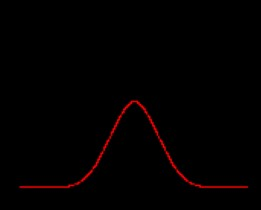
\includegraphics[scale=0.7]{Foto/uc.jpg}
    \color{gray}
    \caption{Uniforme Continua di parametro $U(0,1)$ con n=16}
    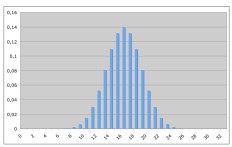
\includegraphics[scale=.9]{Foto/be.jpg}
    \color{gray}
    \caption{Bernoulli di parametro $Be(\sfrac{1}{2})$ con n=32}
    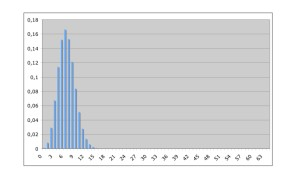
\includegraphics[scale=.8]{Foto/be110.jpg}
    \color{gray}
    \caption{Bernoulli di parametro $Be(\sfrac{1}{10})$ con n=64}
\end{figure}

\newpage
\subsection{Teorema del Limite Centrale}

\ind \textbf{Definizione}: Il \textbf{Teorema del Limite Centrale} (TLC) afferma che la somma o la media di un grande numero di v.a. i.i.d e è approssimativamente normale per n grande ($n \geq 30$). Siano $E[X_i]=\mu$ e $Var[X_i]=\sigma^2$ allora $$ \text{Media: } \pP \left( \dfrac{\mc - \mu}{ \dfrac{\sigma}{\sqrt{n}}} \leq x \right) \sim P(Z \leq x)$$ $$ \text{Somma: } \pP \left( \dfrac{\somsuc - \mu}{ \sigma} \leq x \right) \sim P(Z \leq x)$$

\subsection{Correzioni di Continuità}

\ind \textbf{Definizione}: La correzione di continuità si applica quando si standardizza una distribuzione discreta ad una normale. Afferma che bisogna ampliare di $\sfrac{1}{2}$ gli estremi dell'intervallo per ottenere un valore ben approssimato \n

\ind \textbf{Definizione}: La correzione di continuità di una \textbf{binomiale} afferma che dato se $np \geq 5$ e $n(1 - p) \geq 5$ allora la sua correzione è $$X \sim Bin (np, np(1 - p))$$ 

\ind \textbf{Definizione}: Se non ci troviamo nel caso di prima, quindi $np \leq 5$ e $n(1 - p) \leq 5$ allora approssimiamo con la correzione di continuità di una \textbf{Poisson}: $$X \sim Pois(n(1 - p))$$

%%%%%%%%%%%%%%%%%%%%%%%%%%%%%%%%%%%%%%%%%%%%%%%%%%%%%%%%%%%%%%%%%%%%%%%%%%%%%%%%%%%%%%%%%%%%%%%%%%%%%%%%%%%%%%%%%%%%%%%%%%%%%%%

\newpage
\section{Pratica}

\ind \textbf{Standardizzazione}: $\std$ \n

\ind \textbf{TLC}: $$ \text{Media: } \pP \left( \dfrac{\mc - \mu}{ \dfrac{\sigma}{\sqrt{n}}} \leq x \right) \sim P(Z \leq x)$$ $$ \text{Somma: } \pP \left( \dfrac{\somsuc - \mu}{ \sigma} \leq x \right) \sim P(Z \leq x)$$

\ind \textbf{CC}: Riduzione di $\sfrac{1}{2}$ del dominio per approssimare V.A. discrete \n

\ind \textbf{CC Binomiale}: se $np \geq 5$ e $n(1 - p) \geq 5$ allora: $X \sim Bin (np, np(1 - p))$ \n

\ind \textbf{CC Poisson}: se $np \leq 5$ e $n(1 - p) \leq 5$ allora: $X \sim Pois(n(1 - p))$

\subsection{Esercizi} 

\subsubsection{Esercizio 1: TLC con assolutamente continua}

\textbf{Traccia}: Una lampada ha un tempo di vita che segue una legge esponenziale di media 10 giorni. Non appena la lampada smette di funzionare, viene sostituita con una nuova. 
\begin{enumerate}
    \item [a. ] Qual è la probabilità che 40 lampade siano sufficienti per un anno?
    \item [b. ] Qual è il numero minimo n di lampade comprare affinché la probabilità dell'evento "n lampade siano sufficienti per un anno" sia almeno 0.95?
\end{enumerate} 

\ind \textbf{Soluzione a}: 
\begin{enumerate}
    \item Ricavo dalla traccia che ho 40 lampade con legge esponenziale di media 10 giorni. Ricavo dalla tabella che se $E[X]=\sfrac{1}{\lambda}=10$, allora $\lambda=\sfrac{1}{10}$ Riscrivo come $X_1, ..., X_{40}$ v.a. i.i.d. $\sim exp(\sfrac{1}{10})$
    \item La richiesta è $\pP (X_1 + ... + X_{40} > 365)$. Dato che $n=40$ è abbastanza grande, possiamo stimare questa probabilità con il TLC.
    \item Dobbiamo standardizzare la somma delle nostre v.a. Per farlo abbiamo bisogno di conoscere valore medio $E[X] = \sfrac{1}{\lambda}$ e varianza $Var[X] = \sfrac{1}{\lambda^2}$: 
        \begin{itemize}
            \item Per la linearità della media, $E[X+Y] = E[X] + E[Y]$: $$E[X_1 + ... + X_{40}] = E[X_1] + ... + E[X_{40}] = 10 + ... + 10 = 400$$
            \item Per l'indipendenza delle v.a., $Cov[X+Y]=0$ quindi $Var[X+Y]= Var[X] + Var[Y]$: $$Var[X_1 + ... + X_{40}] = Var[X_1] + ... + Var[X_{40}] = 100 + ... + 100 = 4000$$
        \end{itemize}
    \item Standardizziamo con la formula: $\std$: $$\pP (X_1 + ... + X_{40} > 365) = \pP \left( \dfrac{X_1 + ... + X_{40} - 400}{\sqrt{4000}} > \dfrac{365 - 400}{\sqrt{4000}} \right) $$
        \begin{itemize}
            \item Semplifichiamo e cambiamo $>$ in $\leq$: $$= 1 - \pP \left( \dfrac{X_1 + ... + X_{40} - 400}{\sqrt{4000}} \leq \dfrac{-35}{20\sqrt{10}} \right)$$
            \item Essendo $\sim N(0,1)$ usando il TLC avremo: $$\simeq 1 - \pP \left(Z \leq  \dfrac{-35}{20\sqrt{10}} \right) = 1 -\Phi \left( \dfrac{-35}{20\sqrt{10}} \right)$$  
            \item Essendo l'argomento negativo diventa: $$1 - 1 - \Phi \left( \dfrac{35}{20\sqrt{10}} \right) = \Phi(0.55) = 0.7088$$
        \end{itemize}
    \item La probabilità che 40 lampade siano sufficienti per un anno è 71\%
\end{enumerate}

\ind \textbf{Soluzione b}:
\begin{enumerate}
    \item Abbiamo $X_1 + ... + X_n \sim exp(\sfrac{1}{10})$. L'incognita ora è n. Cerchiamo il minimo n  tc $ \pP(X_1 + ... X_N > 365) \geq 0.95)$
    \item Sicuramente n deve essere $>$ 40 in quanto al punto a. dava probabilità 0.71 e a noi serve 0.95. Essendo n grande, il TLC è applicabile con buona approssimazione.
    \item Dobbiamo standardizzare la somma delle nostre v.a. Calcoliamo valore medio e varianza:
        \begin{itemize}
            \item $E[X_1 + ... + X_n] = E[X_1] + ... + E[X_n] = 10n$
            \item $Var[X_1 + ... + X_n] = Var[X_1] + ... + Var[X_n] = 100n$
        \end{itemize}
    \item Standardizzo: $$ \pP(X_1 + ... + X_n > 365) = 1 - \pP \left( \dfrac{X_1 + ... + X_{n} - 10n}{\sqrt{100n}} \leq \dfrac{365 - 10n}{\sqrt{10\sqrt{n}}} \right)$$
    \item Avrò numeratore negativo perché $n>40$ quindi per TLC: $$\Phi\left(\frac{10n - 365}{10 \sqrt{n}}\right)$$
    \item Calcoliamo il minimo n tc. $$\Phi \left(\frac{10n - 365}{10 \sqrt{n}}\right) \geq 0.95$$
    \item Calcolo con la fdr lo $z^*$ tc $\Phi(z^*) = 0.95$ e trovo $\Phi(1.645)$: $$\Phi\left( \frac{10n - 365}{10 \sqrt{n}}\right) \geq \Phi(1.645) =  \frac{10n - 365}{10 \sqrt{n}} \geq 1.645= \qquad (\sqrt{n} = x)$$  $$= 10x^2 - 16.45x - 365 \geq 0 \xrightarrow{} x=6.92= n \sim 47.89$$ 
    \item Il minimo numero di lampadine da compare è 48
\end{enumerate}

\subsubsection{Esercizio 2: TLC con discreta + CC }

\textbf{Traccia}: Qual è la probabilità di ottenere almeno 29 teste in 50 lanci di una moneta equilibrata? \n

\ind \textbf{Soluzione}: 
\begin{enumerate}
    \item Definiamo $X_1, ..., X_{50} $ v.a. i.i.d $\sim Be(\sfrac{1}{2})$
    \item Cerco il numero di teste nei 50 lanci: $\pP(X_1 + ... + X_{50} \geq 29) $, ovvero $Bin(50, \frac{1}{2})$ con numero di successi $k=29$
    \item Devo usare la CC di una binomiale, dunque devo rispettare due condizioni:
        \begin{enumerate}
            \item $np \geq 5$: $np=50 \cdot \sfrac{1}{2}= 25 \geq 5$
            \item $n(1-p) \geq 5$: $n(1-p)=50\cdot \sfrac{1}{2}=25 \geq 5$
        \end{enumerate}
    \item Essendo entrambe le condizioni confermate, posso approssimare con una binomiale della forma: $$X \sim Bin(np, np(1-p)) = Bin(25, \sfrac{25}{2})$$
    \item Approssimo con la CC ed ottengo: $$\pP(X_1 + ... + X_{50} \geq 28.5) = \pP \left( \dfrac{X_1 + ... + X_{50} - 25}{\sqrt{\dfrac{25}{2}}} \right)$$
    \item Applico il TLC: $$\pP(X_1 + ... + X_{50} \geq 28.5) \sim 1 - \pP \left(Z \leq \frac{7}{\sqrt{50}} \right) = 1 - \Phi(0.99) = 0.1611$$
    \item La probabilità di ottenere almeno 29 teste in 50 lanci è del 16\%
\end{enumerate}



